\section{Related Work}
% 在工程学、物理学、生物学和化学等众多领域,为了解决各种各样的偏微分方程,学术界尝试了非常多的途径,诞生了很多数值解法并且都已经非常成熟。
% 有限差分法是一种被广泛运用的方法,通过差商来近似所需要的连续函数的导数。

To gain well quality solution of various types of PDEs is prohibitive and notoriously challanging.
The number of methods avaliable to determine canonical PDEs is limited as well,
includes 
separation of variables, 
superposition, 
product solution methods, 
Fourier transforms, 
Laplace transforms and 
perturbation methods, 
among a few others.
Even though there methods are exclusively well-performed on constrained conditions,
such as regular shaped geometry domain, constant coefficients, well-symmetric conditions 
and many others.
These limits strongly constrained the range of applicability of numerical techniques for solving PDEs,
rendering them nearly irrelevant for solving problems pratically.

General, the methods of determining numerical solutions of PDEs can be broadly classified into
two types: 
deterministic 
and stochastic. 
The mostly widely used stochastic method for solving PDEs is 
Monte Carlo Method \cite{Monte Carlo Method} which is a popular method in solving PDEs in higher dimension space with 
notable complexity.

\subsection{Finite Difference Method}\label{SEC:FDM}
The Finithe Difference Method(FDM) is based on the numerical approximation method in calculus of finite differences.
The motivation is quiet straightforward which is approximating solutions by finding values satisfied PDEs on a set of 
presctibed interconnected points within the domain of it. Those points are which referd as nodes, and the set of nodes 
are so called as a grid of mesh.
A notable way to approximate derivatives are using 
Taylor Series expansions.
Taking 2 dimension Possion Equation as instance, assuming the investigated value as, $\varphi$,
\begin{equation}\label{EQ_POSSION_2D}
  \frac{
    \partial ^ 2 \varphi  
  }{
    \partial x ^ 2
  } +
  \frac{
    \partial ^ 2 \varphi  
  }{
    \partial y ^ 2
  }
  =  f(x,y)
\end{equation}
The total amount of nodes is denoted with $N = 15$, which gives the numerical equation which governing 
equation \ref{EQ_POSSION_2D} 
shown in 
equation \ref{EQ_POSSION_2D_10_NODES} and nodes layout as shown in the 
figure \ref{FIG_POSSION_2D_10_NODES}
\begin{equation}\label{EQ_POSSION_2D_10_NODES}
  \frac{
    \partial ^ 2 \varphi_i
  }{
    \partial x_i ^ 2
  } +
  \frac{
    \partial ^ 2 \varphi_i
  }{
    \partial y_i ^ 2
  }
  =  f(x_i,y_i) = f_i, \:\:\:\:\: i = 1,2,\dots,15
\end{equation}
\begin{figure}[htbp]
  \centering
  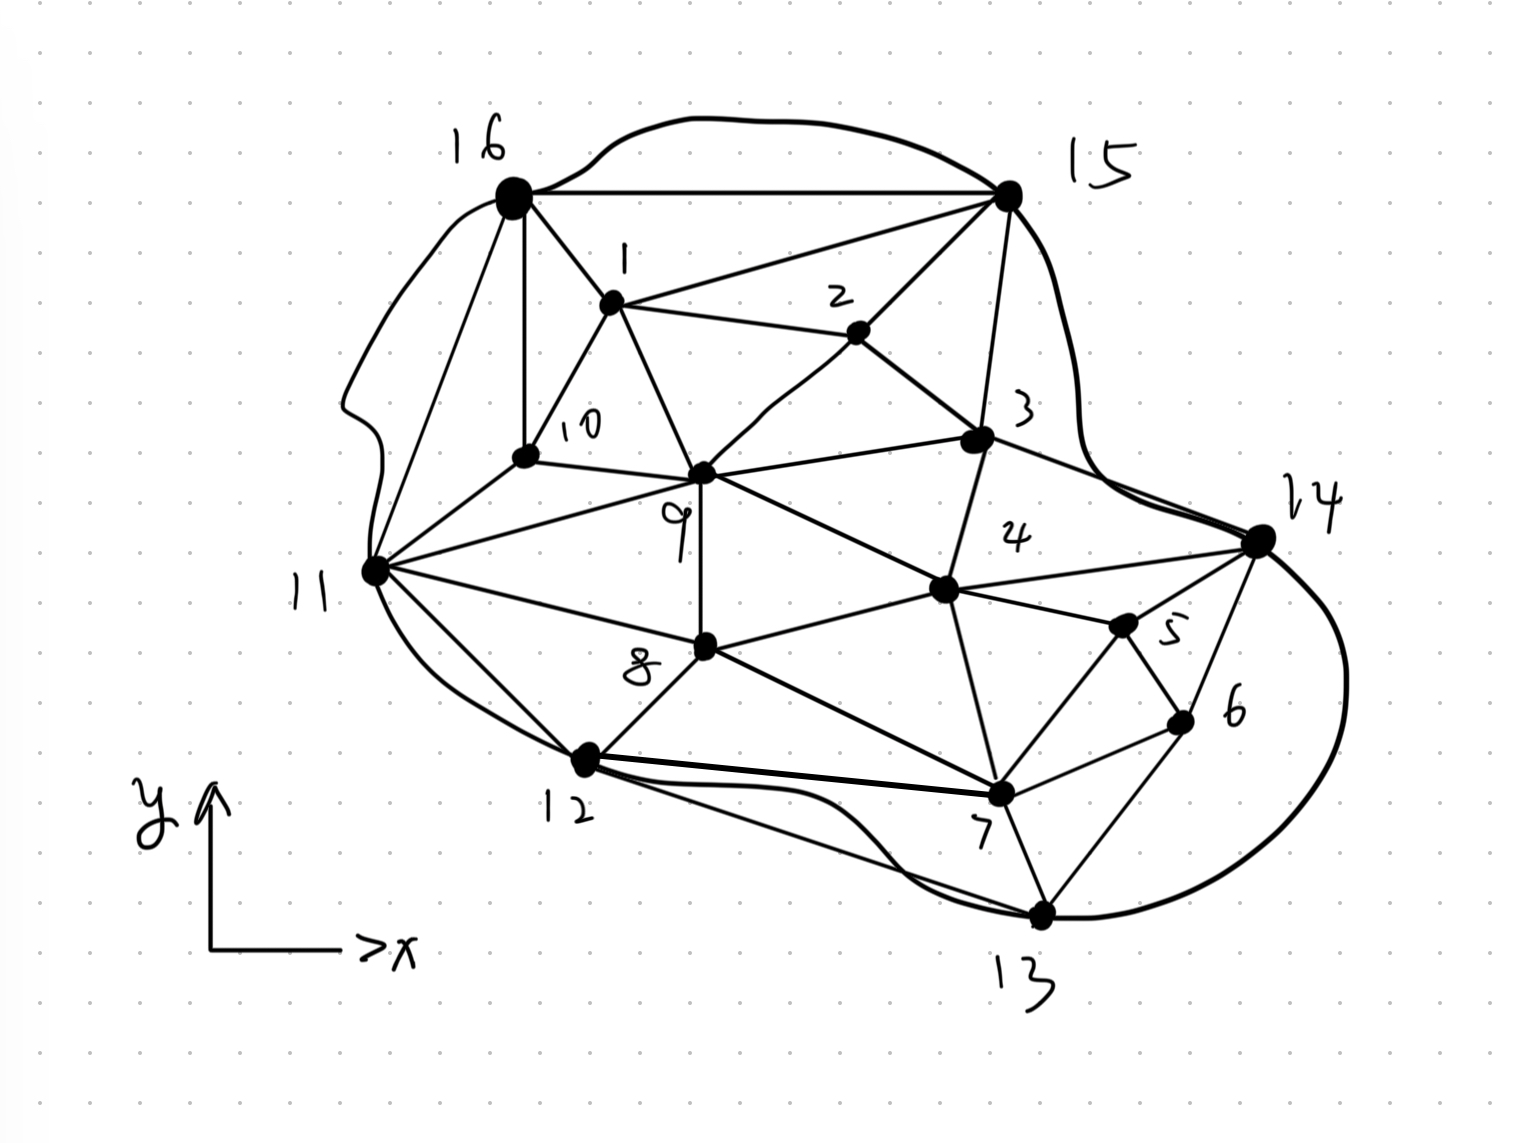
\includegraphics[width=0.5\textwidth]{figure/FIG_POSSION_2D_10_NODES.jpg}
  \caption{The Schematic Representa of of a 2D Computiational Domain and Grid. The nodes are used for the FDM by solid circles. 
  Nodes $11-15$ denote boundary nodes, while nodes $1-10$ denote internal nodes.}
  \label{FIG_POSSION_2D_10_NODES}
\end{figure}
In this case, we only need to find the value of internal nodes which $i$ is ranging from $1$ to $10$.
Next is aimming to solve this linder system \ref{EQ_POSSION_2D_10_NODES}.


\subsection{Physics Informed Neural Networks}
With the explosive growth of avaliable data and computing resouces, 
recent advances in machine learning and data analytics have yieled good results across science discipline, 
including Convolutional Neural Networks (CNNs) \cite{CNN}
for image recoginition, 
Generative Pre-trained Transformer (GPT) \cite{GPT}
for natual language processing and 
Physics Informed Neural Networks (PINNs) \cite{PINN}
for handling science problems with high complexity.
PINNs is a type of machine learning model makes full use of the benefits from 
Auto-differentiation (AD) \cite{AD}
which led to the emergence of a subject called 
Matrix Calculus \cite{Matrix_Calculus}.
Considering the parametrized and nonlinear PDEs of the general form [E.q. \ref{EQ_General_PDEs}] of function $u(t,x)$
\begin{equation}\label{EQ_General_PDEs}
  u_t + \mathcal{N}\left[u;\lambda\right] = 0
\end{equation}
The $\mathcal{N}[\cdot;\lambda]$ is a nonlinear operator which parametrized by $\lambda$.
This setup includes common PDEs problems like heat equation, and black-stokz equation and others.
In this case, we setup a neural network $NN[t,x;\theta]$ which has trainable weights $\theta$ and takes 
$t$ and $x$ as inputs, outputs with the predicting value $\hat{u}(t,x)$.
In the training process, the next step is calculating the necessary derivatives of $u$ with the respect to $t$ and $x$.
The value of loss function is a combination of the metrics of how well does these predictions fit the given conditions and 
fit the natural law [Fig. \ref{FIG_Schematic_View_PINN}]. 
\begin{figure}[htbp]
  \centering
  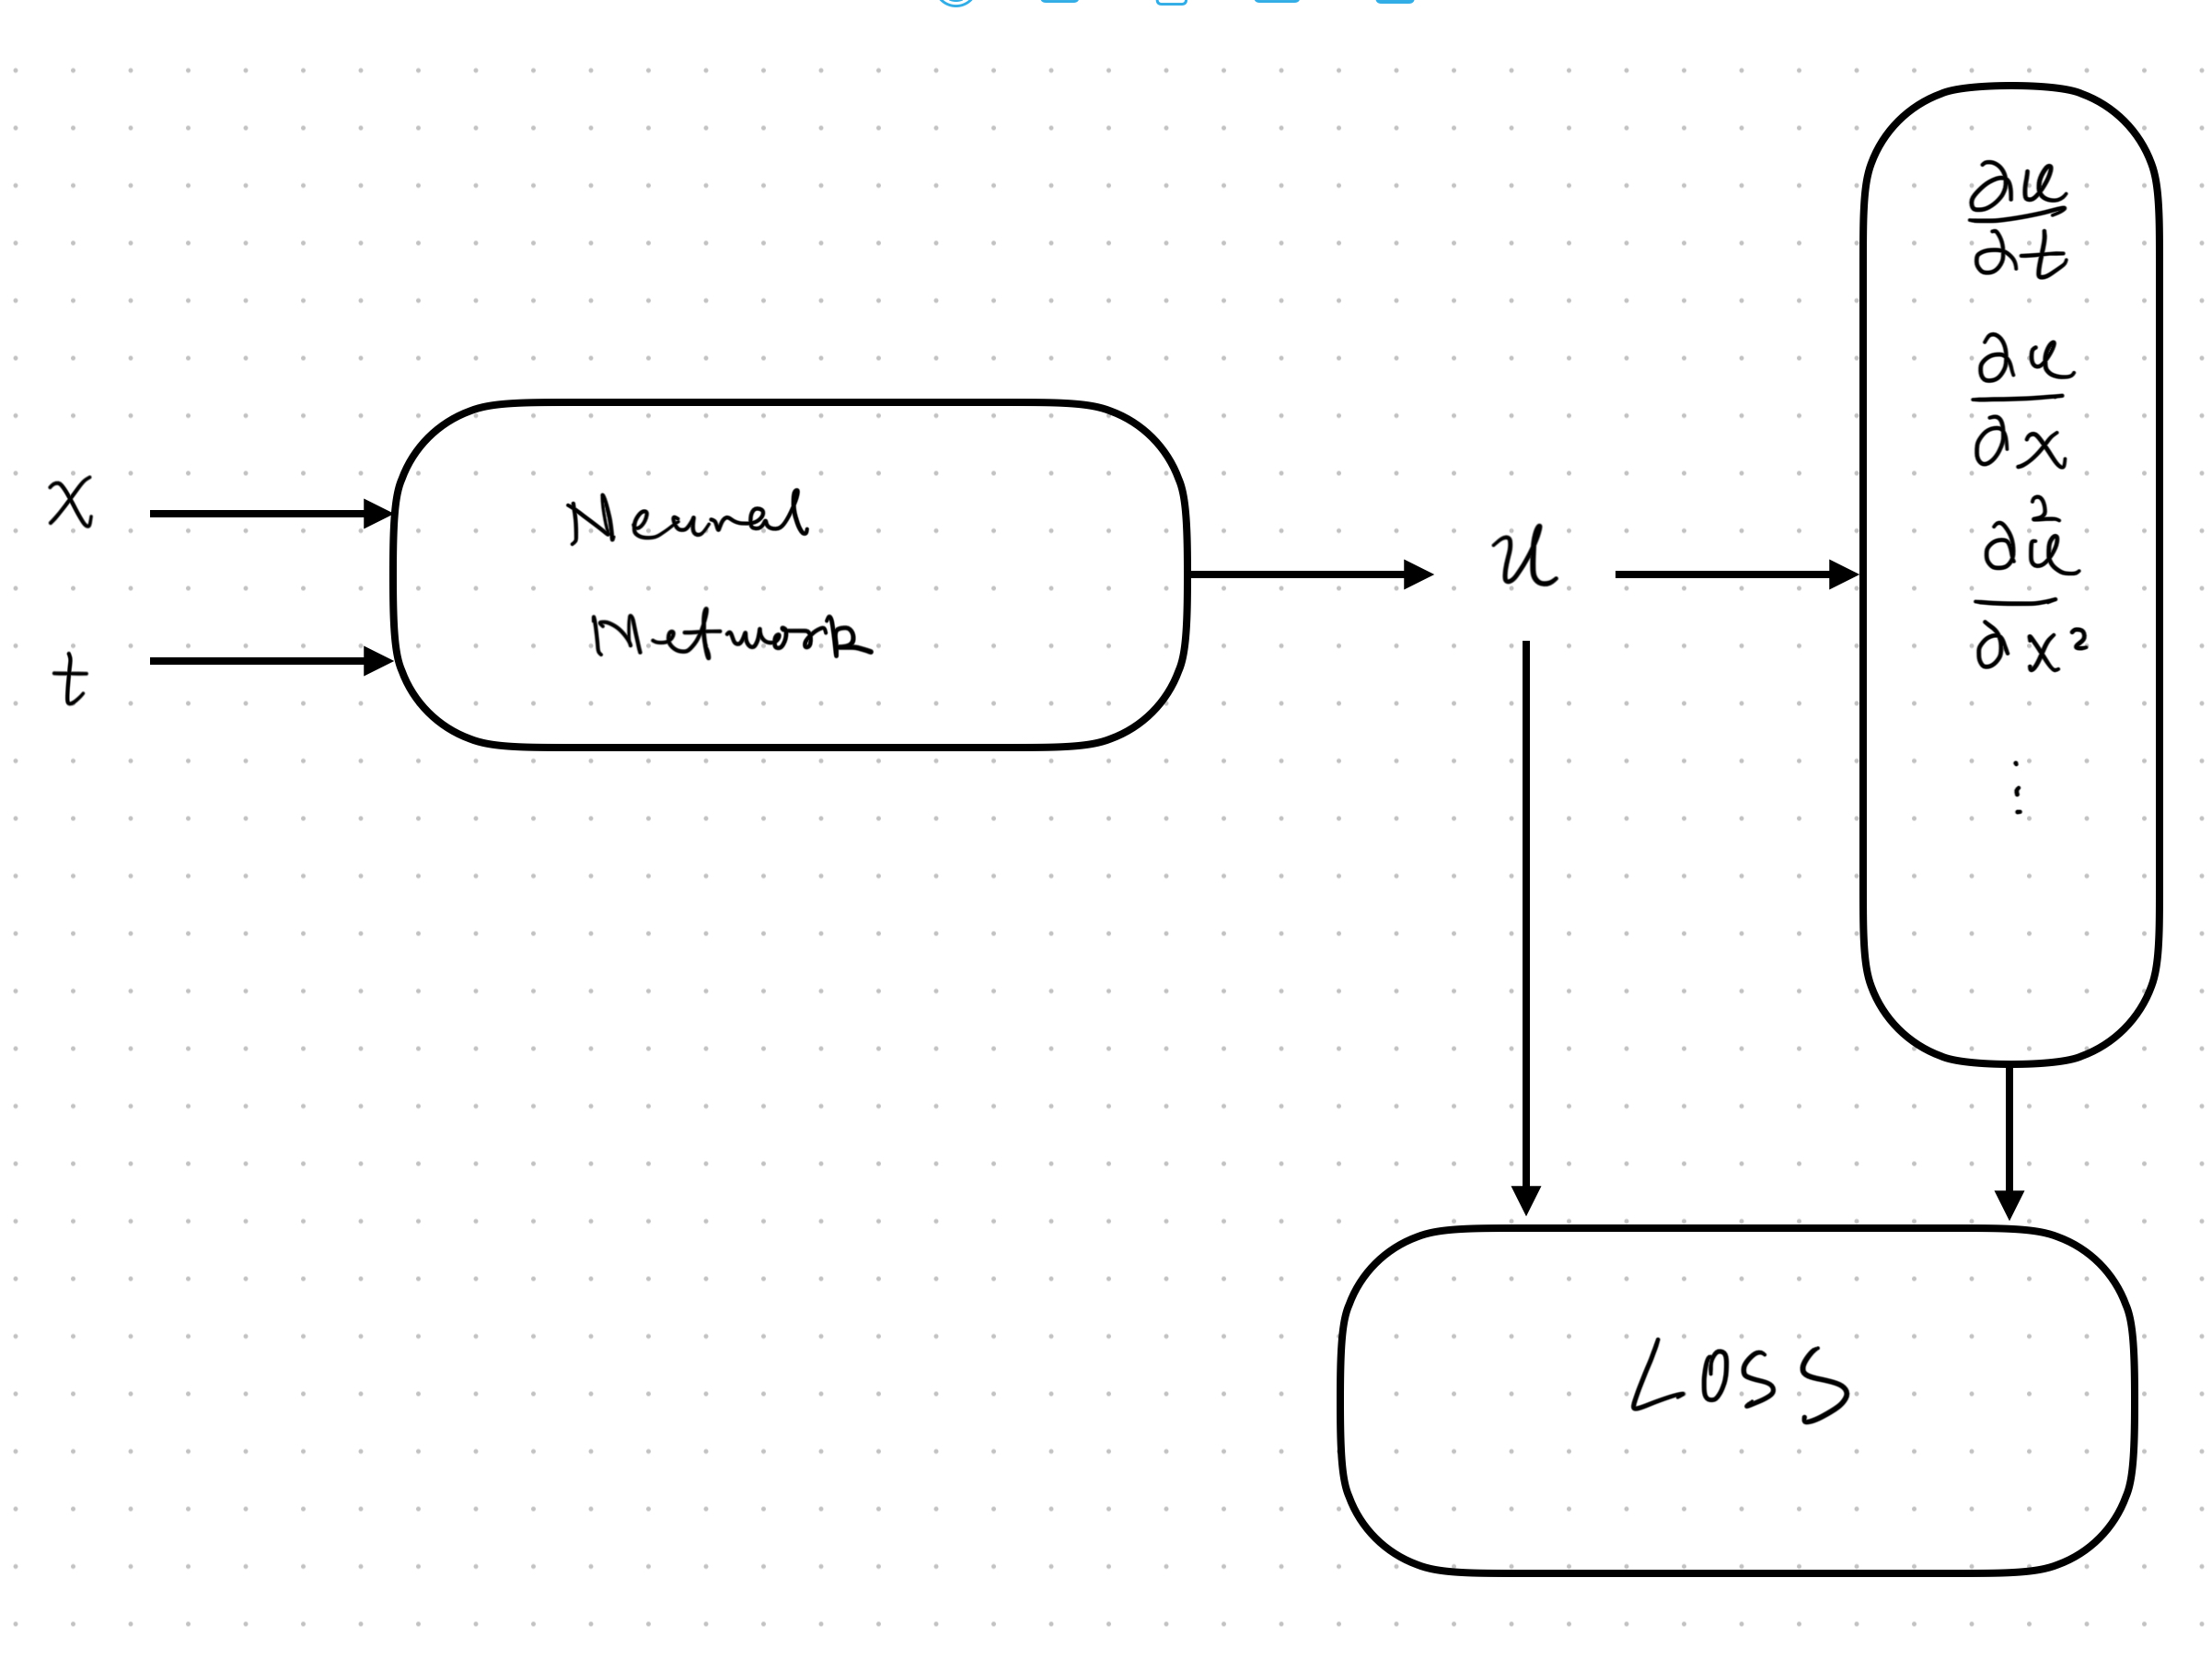
\includegraphics[width=0.5\textwidth]{figure/FIG_Schematic_View_PINN.jpg}
  \caption{The Schematic Representa of a structure of PINN.}
  \label{FIG_Schematic_View_PINN}
\end{figure}

\subsection{Finite Difference Time Domain Method}
As described previously in the 
section \ref{SEC:FDM}, FDM could solve the PDEs in its original form where 
Finite Element and Finite Volume Methods gained results by solving modified form such as an integral form of the governing equation.
Though the latter methods are commonly get better results or less computational hungery, 
the FDM has many descendants, 
for instance the Finite Difference Time Domain Method (FDTD) where it still finds prolific usage are computational heat equation and 
computational electromagnetics (Maxwell's equations \cite{Maxwell_equations}). 
Assuming the operator $\mathcal{N}[\cdot;\lambda]$ is set to $\nabla$ where it makes E.q. \ref{EQ_General_PDEs} become 
to heat equation \ref{EQ_HEAT_EQ_EG}.
\begin{equation}\label{EQ_HEAT_EQ_EG}
  \frac{\partial u}{\partial t} 
  - \lambda \left(
    \frac{\partial^2 u}{\partial x^2}  + \frac{\partial^2 u}{\partial y^2} 
  \right) = 0
\end{equation}
Using the key idea of FDM, assuming the step size in spatio-time space are $\Delta x$, $\Delta y$ and $\Delta t$,
we could have a series equations which have form [E.q. \ref{EQ_FDM_FDTD_EQ}].
\begin{equation}\label{EQ_FDM_FDTD_EQ}
  \frac{u^{n+1}_{i,j} - u^n_{i,j}}{\Delta t} 
  = 
  \lambda
  \left(
    \frac{
      u^n_{i+1,j} - 2u^n_{i,j} + u^n_{i-1,j}
    }{\Delta x^2}
    +
    \frac{
      u^n_{i,j+1} - 2u^n_{i,j} + u^n_{i,j+1}
    }{\Delta y^2}
  \right)
\end{equation}
when the time step size satisfies the 
Couran, Friedrichs, and Lewy condition (CFL\cite{CFL_limitation}).
We could get the strong results by iterating the equation \ref{EQ_FDM_FDTD_EQ}, or more specifically using 
equation \ref{EQ_FDM_FDTD_EQ_Iterating} to get the value $u$ of next time stamp $n+1$ on nodes $i,j$.
\begin{equation}\label{EQ_FDM_FDTD_EQ_Iterating}
  u^{n+1}_{i,j}
  = 
  u^n_{i,j} + 
    \frac{
      \lambda\Delta t
    }{\Delta x^2}\left(
      u^n_{i+1,j} - 2u^n_{i,j} + u^n_{i-1,j}
    \right)
    +
    \frac{
      \lambda\Delta t
    }{\Delta y^2}\left(
      u^n_{i,j+1} - 2u^n_{i,j} + u^n_{i,j+1}
    \right)
\end{equation}
also shown in the figure \ref{FIG_Schematic_View_FDTD}.
\begin{figure}[htbp]
  \centering
  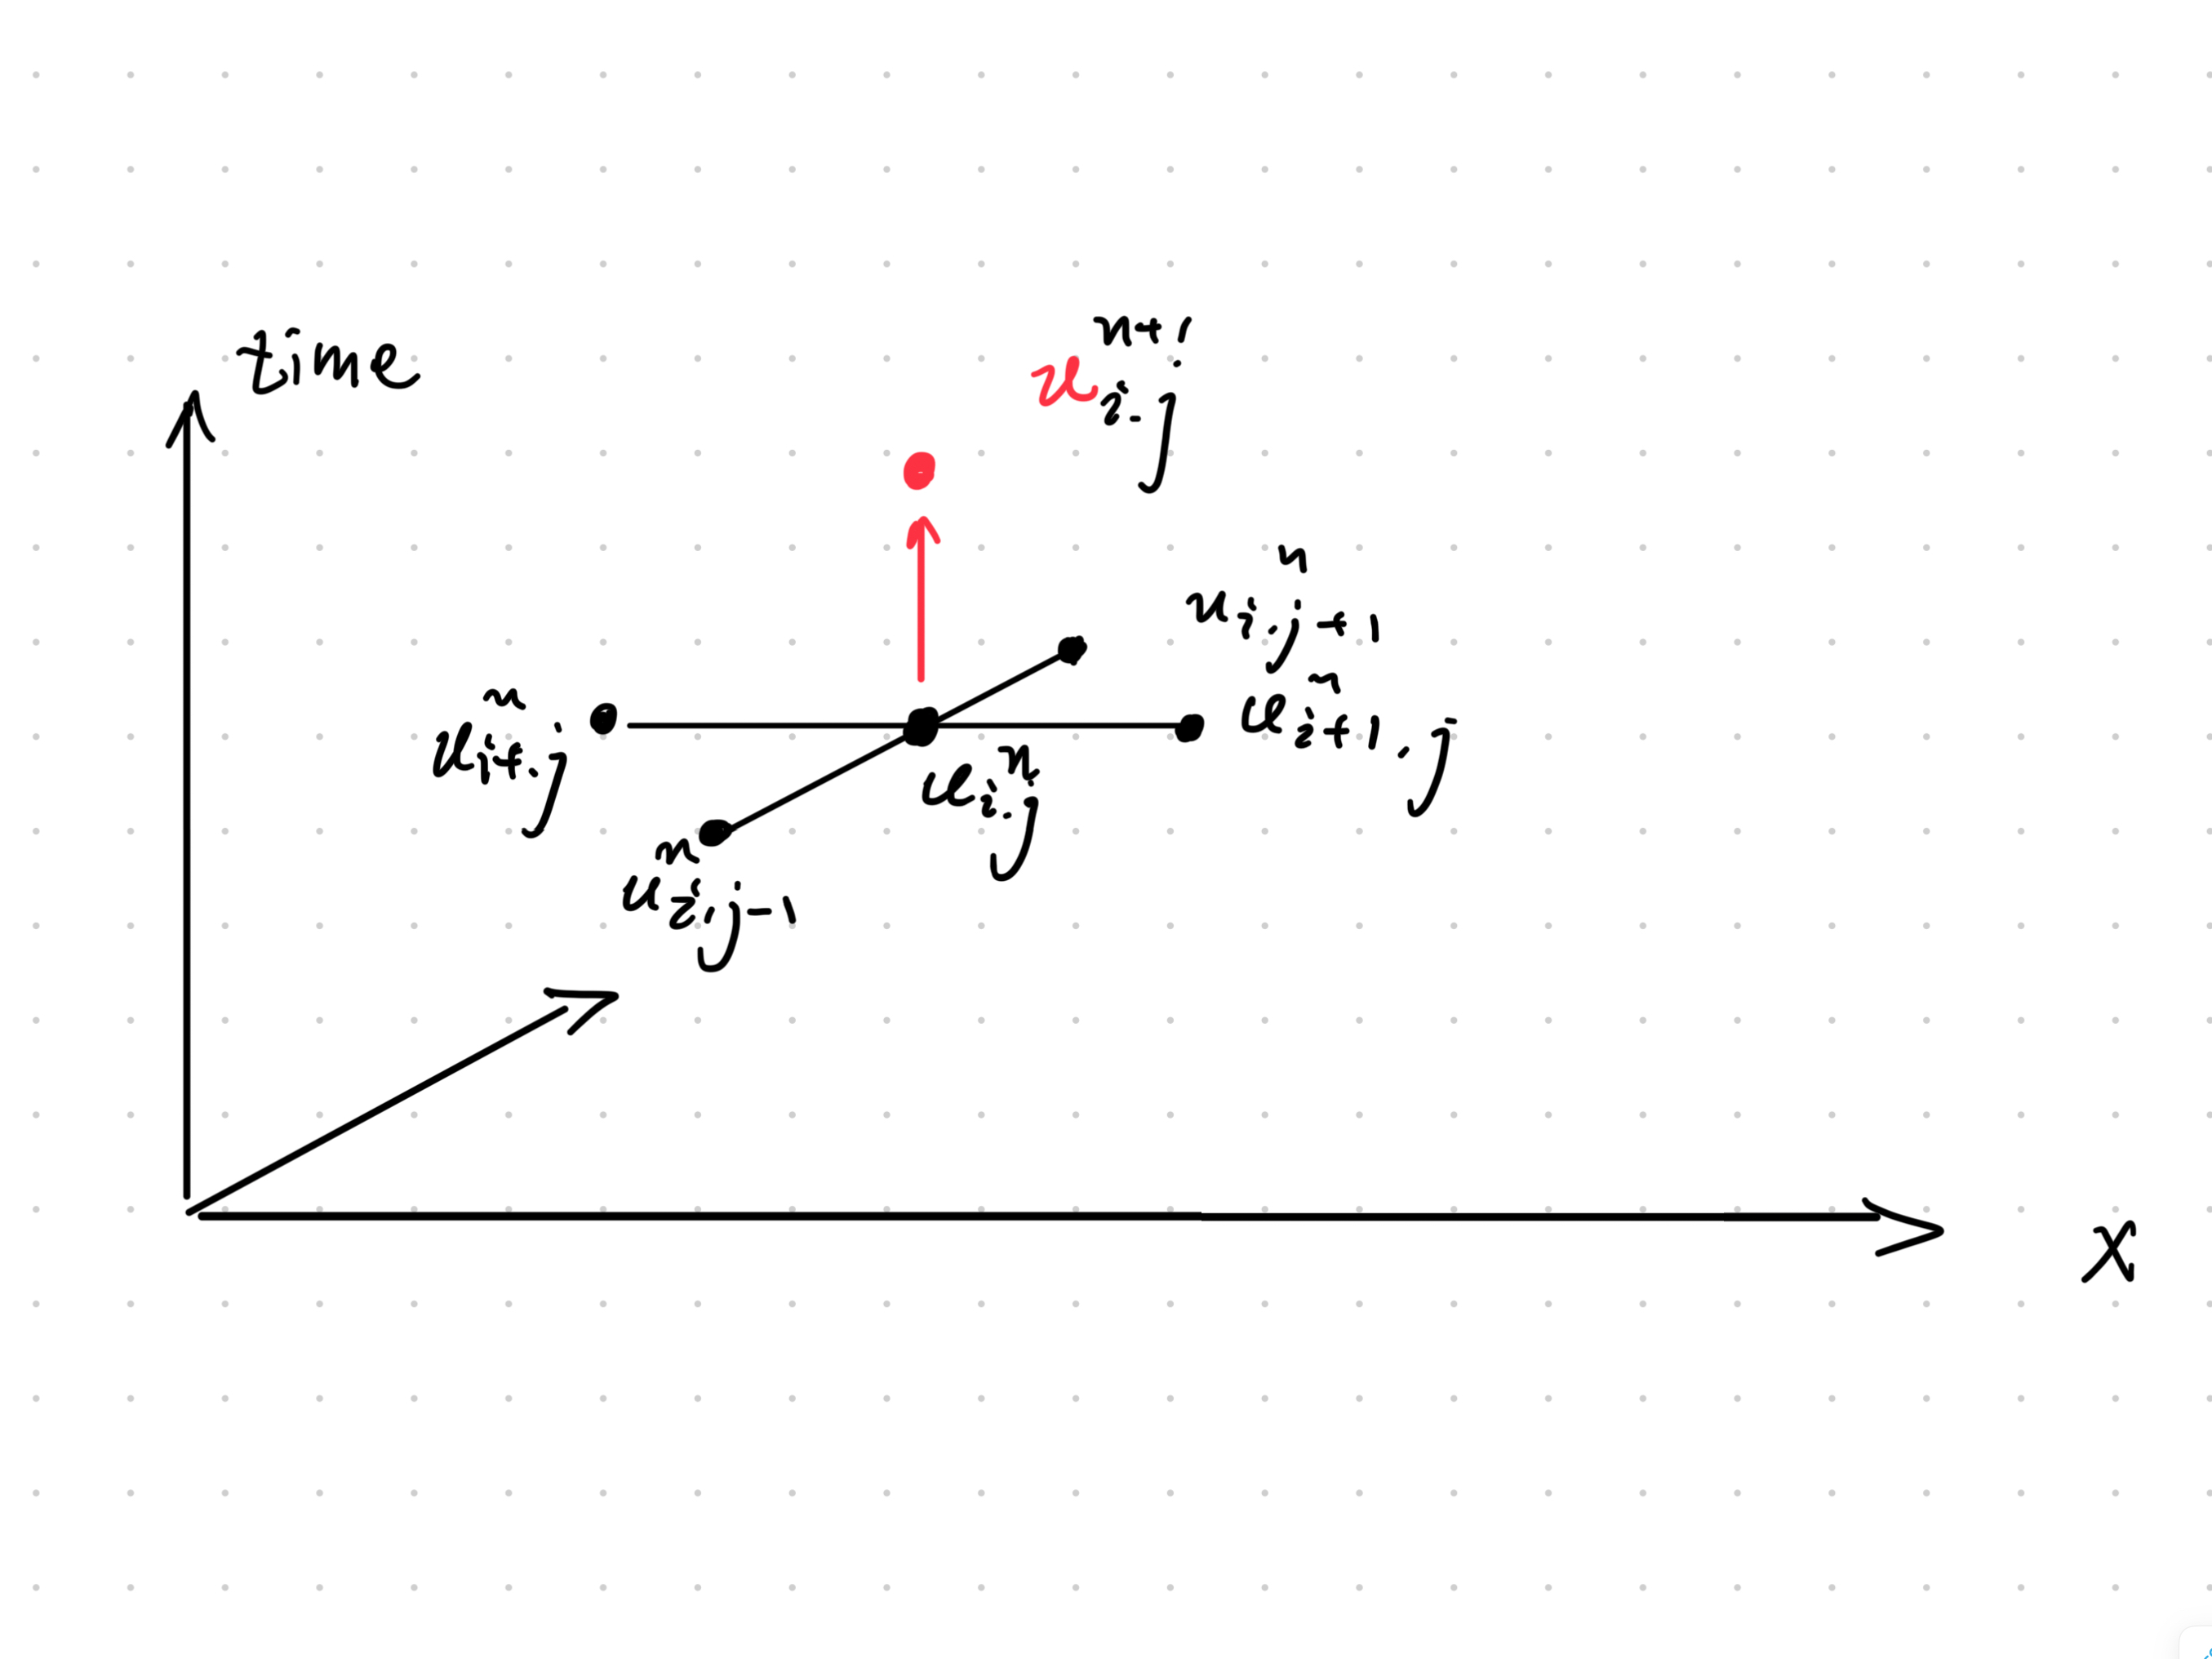
\includegraphics[width=0.5\textwidth]{figure/FIG_Schematic_View_FDTD.jpg}
  \caption{The Schematic Representa the computational spatio-time domain of FDTD methods.}
  \label{FIG_Schematic_View_FDTD}
\end{figure}


